\documentclass[paper=a4, fontsize=11pt]{scrartcl} % A4 paper and 10pt font size
\usepackage[T1]{fontenc} % Use 8-bit encoding that has 256 glyphs
%\usepackage{fourier} % Use the Adobe Utopia font for the document - comment this line to return to the LaTeX default
\usepackage[english]{babel} % English language/hyphenation
\usepackage{lscape}
\usepackage{mathptmx}
\usepackage{url}
\usepackage{sectsty} % Allows customizing section commands
\setlength{\columnsep}{5mm}
\usepackage{natbib}
\usepackage{setspace}
\usepackage{lipsum}
\usepackage{amsmath}
\usepackage{relsize}
\usepackage{eurosym}
\usepackage[most]{tcolorbox}
\usepackage{inconsolata}
 \usepackage{booktabs}
\newtcblisting[auto counter]{sexylisting}[2][]{sharp corners, 
    fonttitle=\bfseries, colframe=gray, listing only, 
    listing options={basicstyle=\ttfamily,language=R}, 
    title=Listing \thetcbcounter: #2, #1}
\title{MIS40520 Analytics Business Modelling - Assignment 1}

\DeclareOldFontCommand{\rm}{\normalfont\rmfamily}{\mathrm}
\DeclareOldFontCommand{\sf}{\normalfont\sffamily}{\mathsf}
\DeclareOldFontCommand{\tt}{\normalfont\ttfamily}{\mathtt}
\DeclareOldFontCommand{\bf}{\normalfont\bfseries}{\mathbf}
\DeclareOldFontCommand{\it}{\normalfont\itshape}{\mathit}
\DeclareOldFontCommand{\sl}{\normalfont\slshape}{\@nomath\sl}
\DeclareOldFontCommand{\sc}{\normalfont\scshape}{\@nomath\sc}
\DeclareRobustCommand*\cal{\@fontswitch\relax\mathcal}
\DeclareRobustCommand*\mit{\@fontswitch\relax\mathnormal}

%----------------------------------------------------------------------------------------
%	Caption Set & URL Font Control
%----------------------------------------------------------------------------------------
\usepackage[font=footnotesize,labelfont=bf]{caption}
\captionsetup{justification=centering}
\usepackage{subcaption}
\urlstyle{rm}
\usepackage{authblk}

\usepackage{geometry}
 \geometry{
 a4paper,
 total={170mm,257mm},
 left=20mm,
 top=20mm,
 footskip=10mm
 }

\usepackage{graphicx}
\graphicspath{ {images/} }
\usepackage{indentfirst}
\usepackage{dirtree}
\setlength\parindent{0pt} % Removes all indentation from paragraphs - comment this line for an assignment with lots of text

%----------------------------------------------------------------------------------------
%	Header Footer
%----------------------------------------------------------------------------------------
\usepackage{fancyvrb}
\usepackage{fancyhdr}
\pagestyle{fancy}
\lhead{MIS40520: Analytical Business Modelling}
\rhead{Shruti Goyal \\ Deepak Kumar Gupta}
\cfoot{\thepage}

%----------------------------------------------------------------------------------------
%	TITLE SECTION
%----------------------------------------------------------------------------------------
\begin{document}
\begin{titlepage}
\newcommand{\HRule}{\rule{\linewidth}{0.5mm}} % Defines a new command for the horizontal lines, change thickness here
\center % Center everything on the page

%----------------------------------------------------------------------------------------
%	HEADING SECTIONS
%----------------------------------------------------------------------------------------
\textsc{\LARGE UCD Michael Smurfit Graduate Business School}\\[1.7cm] % Name of your university/college

\includegraphics[scale = 0.7]{logo.png} \\ [1cm]
\textrm{\Large	\textrm{MIS40520: Analytical Business Modelling}}\\[0.6cm] % Major heading such as course name

%----------------------------------------------------------------------------------------
%	TITLE SECTION
%----------------------------------------------------------------------------------------

\HRule \\[0.5cm]
{ \LARGE  \textrm{M(I)LP Assignment 2}}\\[0.5cm] % Title of your document
\HRule \\[1.5cm]
 
%----------------------------------------------------------------------------------------
%	AUTHOR SECTION
%----------------------------------------------------------------------------------------

\begin{minipage}{0.45\textwidth}
\begin{flushleft} \large
\emph{\textrm{Authors:}}\\
\normalsize{Goyal \textrm{Shruti} (16200726)}\\
\normalsize{Gupta \textrm{Deepak Kumar} (16200660) }\\
\end{flushleft}
\end{minipage}
~
~
\begin{minipage}{0.45\textwidth}
\begin{flushright} \large
\emph{\textrm{Lecturer:}} \\
\normalsize{Dr Paula \textrm{Carroll}} % Supervisor's Name
\end{flushright}
\end{minipage}\\[3cm]
% If you don't want a supervisor, uncomment the two lines below and remove the section above
%\Large \emph{Author:}\\
%John \textsc{Smith}\\[3cm] % Your name

%----------------------------------------------------------------------------------------
%	DATE SECTION
%----------------------------------------------------------------------------------------
\vspace{3cm}
{\large \today}\\[1cm] % Date, change the \today to a set date if you want to be precise
\vfill % Fill the rest of the page with whitespace
\end{titlepage}

%% Begin Writing the Document

%----------------------------------------------------------------------------------------
%	MAIN BODY
%----------------------------------------------------------------------------------------
%\setlength{\parindent}{10ex}
%Context

%\pagenumbering{roman}
%\tableofcontents
%\listoffigures
%\listoftables
%\addcontentsline{toc}{section}{Executive Summary}
%\cleardoublepage
%\clearpage

%----------------------------------------------------------------------------------------
%	EXECUTIVE SUMMARY
%----------------------------------------------------------------------------------------
\subtitle{\normalsize{Optimal Solution for Conference Management}}
\title{Executive Summary}
\author{\small{Shruti Goyal, Deepak Kumar Gupta and Dr Paula Carroll}}
\date{}
\maketitle

Out of 185 available rooms in 10 four star hotel, 150 rooms allocated allocated to delegates using M(I)LP, Mixed integer linear programming optimization model. For given business problem for minimizing organiser cost while maintain average satisfactory rating of each hotel ,minimum cost found is \euro 16207 subject to given constraints and average customer satisfaction rating is 8.30067 for this solution.
\\
% Please add the following required packages to your document preamble:
% \usepackage{booktabs}
\begin{table}[ht]
\centering
\begin{tabular}{@{}lccccccccccc@{}}
\toprule
Hotel Index                             & 1                       & 2                       & 3                        & 4                        & 5                        & 6                       & 7                        & 8                       & 9                        & 10                       & Total                    \\ \midrule
\multicolumn{1}{|l|}{Price ( Euro )}    & \multicolumn{1}{c|}{89} & \multicolumn{1}{c|}{99} & \multicolumn{1}{c|}{119} & \multicolumn{1}{c|}{112} & \multicolumn{1}{c|}{143} & \multicolumn{1}{c|}{94} & \multicolumn{1}{c|}{130} & \multicolumn{1}{c|}{98} & \multicolumn{1}{c|}{155} & \multicolumn{1}{c|}{152} & \multicolumn{1}{c|}{-}   \\ \midrule
\multicolumn{1}{|l|}{Room Availability} & \multicolumn{1}{c|}{35} & \multicolumn{1}{c|}{30} & \multicolumn{1}{c|}{15}  & \multicolumn{1}{c|}{15}  & \multicolumn{1}{c|}{15}  & \multicolumn{1}{c|}{20} & \multicolumn{1}{c|}{15}  & \multicolumn{1}{c|}{10} & \multicolumn{1}{c|}{10}  & \multicolumn{1}{c|}{20}  & \multicolumn{1}{c|}{185} \\ \midrule
\multicolumn{1}{|l|}{Room Allocated}    & \multicolumn{1}{c|}{35} & \multicolumn{1}{c|}{30} & \multicolumn{1}{c|}{6}   & \multicolumn{1}{c|}{15}  & \multicolumn{1}{c|}{0}   & \multicolumn{1}{c|}{20} & \multicolumn{1}{c|}{15}  & \multicolumn{1}{c|}{10} & \multicolumn{1}{c|}{10}  & \multicolumn{1}{c|}{9}   & \multicolumn{1}{c|}{150} \\ \midrule
Cost                            & \euro 3115                    & \euro 2970                    & \euro 714                      & 1680                     &  \euro 0                        & \euro 1880                    & \euro 1950                     & \euro 980                     &  \euro 1550                     & \euro 1368                     & \euro 16207                    \\ \bottomrule
\end{tabular}
\caption{Number of Rooms allocated to Delegates in each Hotel}
\label{my-label}
\end{table}

\begin{figure}[ht]
\centering
\begin{subfigure}{.5\textwidth}
  \centering
  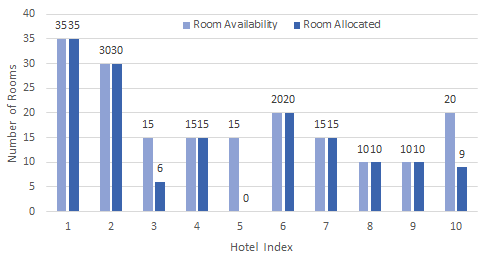
\includegraphics[scale=0.65]{es1.png}
  \caption{Rooms Availability vs Allocated }
  \label{fig:sub1}
\end{subfigure}%
\begin{subfigure}{.5\textwidth}
  \centering
  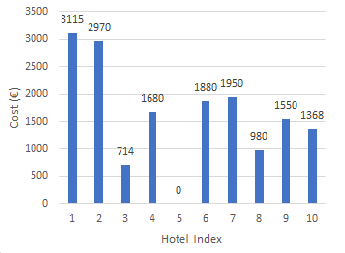
\includegraphics[scale=0.65]{es2.png}
  \caption{Total Cost for Each Hotel (\euro)}
  \label{fig:sub2}
\end{subfigure}
\caption{ Optimal cost and number of rooms allocated } 
\label{fig:es}
\end{figure}
\clearpage	
%----------------------------------------------------------------------------------------
%	BACKGROUND
%----------------------------------------------------------------------------------------
\section{Background}
You have been asked to help organise hotel accommodation for 150 delegates
attending a conference in UCD. You use a hotel booking website to extract the data
shown in the Table below for ten four star hotels in Dublin city centre. The Table
shows the price for a single room per person per night, the customer satisfaction
rating and the number of rooms available for each hotel. The conference organisers
want to allocate the delegates to hotels at minimum cost while achieving an average
customer satisfaction rate of at least 8.3. Formulate an (I)LP model of this problem. 

\begin{table}[ht]
\centering
\begin{tabular}{@{}|l|l|l|l|l|l|l|l|l|l|l|@{}}
\toprule
Hotel Index       & 1   & 2   & 3   & 4   & 5   & 6   & 7   & 8   & 9   & 10  \\ \midrule
Price (\euro)     & 89  & 99  & 119 & 112 & 143 & 94  & 130 & 98  & 155 & 152 \\ \midrule
Customer rating   & 7.8 & 8.3 & 8   & 8.7 & 8   & 8.1 & 8.6 & 8.9 & 8.9 & 8.4 \\ \midrule
Room Availability & 35  & 30  & 15  & 15  & 15  & 20  & 15  & 10  & 10  & 20  \\ \bottomrule
\end{tabular}
\caption{Hotel Data}
\label{hoteldata}
\end{table}
%----------------------------------------------------------------------------------------
%	METHODOLOGY
%----------------------------------------------------------------------------------------


%----------------------------------------------------------------------------------------
%	INTRODUCTION
%----------------------------------------------------------------------------------------

\section{Introduction}

Operation research provides mathematical programming techniques for solving real life problems subject to constraints. Whereas linear programming uses the basis mathematical programming for a linear equation objective function $f(z)$ and a set of constraints equations which are set of linear inequalities or equality  constraints.
\\
\\
An integer (linear) programming (IP) problem is a linear programming problem in which some or all of the decision variables are restricted to be integer valued. In some real scenarios we can not allocate fractional of something, for example: 3 $\frac{1}{2}$ teachers required for a class of 100 students, but 3 $\frac{1}{2}$ teachers is not possible. That is why we require integer (linear) programming for solving such real life problems.
\\

\subsection{Research Paper Review: 1}
Li, Yihua, Qing Miao, and Bruce X. Wang. "Modeling a cruise line revenue management problem." Journal of Revenue and Pricing Management 13.3 (2014): 247-260. \\

In last 3 decades, Cruise line has seen tremendous increase in number of customers, fleet size of cruise etc. however, this segment received less focus from researcher on revenue optimization. Over last 10 years, average price has decreased due to increase in cruise line and competition among different service provider. Cruise line has some similarity with hotel and airline industry, but cruise line has different pricing model and higher occupancy rate. Here, Objective is to maximize the Cruise revenue by sales of rooms for each sailing. Pricing for a room in Cruise is per person basis because cruise has to make additional arrangement per person in terms of food, consumptions etc, whereas in Hotel there is marginal difference between single bed room and double room fare. \\

\textbf{Methods:}\\
Dynamic Programming is not suitable for this case because it take longer time to process and difficult to manage with multiple dependent constraints. Therefore, Linear (integer) programming is best optimization model for this case using linear objective equations and linear constraints equations. This model can be repeatedly applied for capacity allocation and pricing. problem formulation with linear equations and constraint equations has 648 binary variables and 648 non negative variables along with 852 constraints.\\

\textbf{Limitations in Cruise line industry:}\\
1. Ship do not accept more than 2.5 or 3 person per room\\
2. Number of total seats on lifeboats\\
3. Number of rooms available for each room category\\

\textbf{Comparison with Conference Management business problem: }\\
Cruise line revenue management require integer programming as room can not booked in fractions. Each cruise ship has 800 rooms, and each room is classified into 12 segment according to its size, location, view, capacity etc. Guests are charged according of three types of fare: Double occupancy (DO), extra adults(XA), and extra child (XC) with each fare type has 18 fare tiers.\\

Here, we can relate Hotel Index in Conference management problem with room segments, rating of each hotel room with its segment factors i,e size, location, view and room availability is similar to number of available rooms under each segment. However, Cruise line problem is about maximizing the revenue and pricing, whereas conference management problem about minimizing cost while achieving average customer satisfaction rating.

\subsection{Research Paper Review: 1}
Baur, A., Klein, R. \& Steinhardt, C. OR Spectrum (2014) 36: 557. doi:10.1007/s00291-013-0338-3 \\ \\
TUI Deutschland is the Germany's leading tour operator organisation who wants to design its tour operator brochure for optimal hotel room prices which will be valid for atleast 6 months. The task of determining hotel room prices is being done manually by number of specialists; who are responsible for setting of 100,000 prices. The objective of the paper is to develop a decision support system to accomplish the task without much manual effort.\\ 

Paper states that majority of the customers buy holiday packages via brochures that they can get from their local agencies and can choose their desired holiday. While setting prices some factors have to be considered such as purchase prices, hotel ratings, competitor offerings and customer preferences. Before publishing brochures, specialist have to consider following for every hotel : \\ \\
1. Total number of seasons to be displayed\\
2. Price of each room according to season\\
3. How to assign a season to each day \\ \\
Major challenge specialist faced is to finding a trade off between maximum profit and easily understandable price brochure. \\ \\
\textbf{Methods:}
\\ \\
Earlier while developing pricing model, pricing specialists focuses more on customer preferences and their demand. Whereas, paper presented a different approach by taking into account customer's choice that can be estimated from past data. Paper has combined two approaches i.e. predictive analytics and prescriptive analytics : \\
1. \textbf{Predictive Analytics} aims at customer choice and demand dependencies for different hotel and room alternatives, to determine price optimization. Demand for a product has been calculated by dividing its attractiveness by sum of attractiveness of all available options. \\
2. \textbf{Prescriptive Analytics} focuses on optimization techniques and models. Paper has introduced fractional mixed integer programming to optimized sum of ratios.  \\ 

\textbf{Comparison with Conference Management business problem: }\\ \\
Paper introduced mixed integer programming model for determining price optimization process for tour brochures while taking into account customer demand, hotel ratings, room prices; which is similar to conference management problem that is also based on M(I)LP model constraints to hotel ratings, hotel room prices and room availability. MIP model for pricing strategy is a two fold decision support system which also examine behaviour of the model in practice i.e. number of decision support scenarios. Model first has been formulated into general MIP model by defining few additional variables for specific day and customer segments and then reformulated the model based on season type. \\ \\
So, overall objective of the Brochure Price Process model is to calculate a single price strategy model for all hotel room types that can be published in the brochure for maximising sales of the holiday packages. Whilst, conference management model aims at minimising cost in order to accommodate all delegates at the given hotels. Though both the models are somewhat similar based on the type of the model used and similar constraints.

\section{Methodology}


Assumptions:
\begin{itemize}
\item Hotel Index is non-negative index number and always start from 
\item Price of each hotel is always non \- zero and non\-negative 
\item There are only 10 four star hotel and there is no other hotel, where delegates can stay
\item It is assumed that room booking is confirmed and non-refundable, while calculating final cost
\item It is assumed that hotel has flat price for each room, irrespective of length for which delegates stay in hotel
\item All other cost such as food consumption, chauffeur, laundry service etc is not considered while calculating optimal cost


\item Proportionality - The contribution of each decision variable
to the objective or constraint is directly proportional to the
value of the decision variable.
\item Additivity - The contribution to the objective function or
constraint for any variable is independent of the values of the
other decision variables, and the terms can be added together.
\item Divisibility - The decision variables are continuous and thus
can take on fractional values.
\item Deterministic - All the parameters (objective function
coefficients, right-hand side coefficients, left-hand side, or
technology, coefficients) are known with certainty
\end{itemize}

We have total delegates 150 and 10 four star hotels to accommodate guests. We need to minimize the cost while achieving minimum average rating of 8.3:\\

Lets say $HI$ as $Hotel$ $Index$, $devVar(HI)$ as decision variable, $Avail$ as Room Availability and $Rating$ as Customer rating:\\

\textbf{Resource Availability:}
\begin{itemize}
\item 150 delegates
\item 10 four star hotels in city center
\item 185 rooms available to allocate
\end{itemize}
\begin{equation}
decVar(HI) ,\ where\ HI = 1,2,3,4,5,6,7,8,9,10
\end{equation}

\textbf{Decision Variables:} 10 decision variables for each hotel index (HI)
\begin{equation}
decVar(HI) ,\ where\ HI = 1,2,3,4,5,6,7,8,9,10
\end{equation}

\textbf{Objective Function:} 

\begin{equation}
‎‎Cost‎ ‎=‎ \mathlarger{\mathlarger{‎‎\sum}}_{HI=1}^{10}{Price(HI)* decVar(HI}
\end{equation}
\begin{equation}
minimize{(Cost)},\ \text{cost for allocating hotel room to 150 delegates}
\end{equation}


\textbf{ Resource Constraint:} \\

Achieving  average customer satisfaction rating of at least 8.3 while allocating room to delegates, 
\begin{equation}
Avg. Rating ‎=‎ \frac{\mathlarger{\mathlarger{‎‎\sum}}_{HI=1}^{10}{Rating(HI)*decVar(HI))}}{150} \leq 8.3
\end{equation}
\\Coefficient of  each decision variable should be less than equal to room availability in each hotel
\begin{equation}
decVar(HI) <= Avail(HI), HI \in \{1,10\}
\end{equation}

\textbf{Non-negative and Integer Constraint:}\\

Coefficient of each decision variable is integer and non-negative 
\begin{equation}
		decVar(i)\ is\_integer
\end{equation}
\begin{equation}
		decVar(i)>=0
\end{equation}

%----------------------------------------------------------------------------------------
%	RESULTS AND ANALYSIS
%----------------------------------------------------------------------------------------

\section{Analysis of Results}

\begin{table}[ht]
\centering
\begin{tabular}{@{}ccc@{}}
\toprule
\textbf{Hotel Index}     & \textbf{LP Model}         & \textbf{(I)LP Model}    \\ \midrule
\multicolumn{1}{|c|}{1}  & \multicolumn{1}{c|}{35}   & \multicolumn{1}{c|}{35} \\ \midrule
\multicolumn{1}{|c|}{2}  & \multicolumn{1}{c|}{30}   & \multicolumn{1}{c|}{30} \\ \midrule
\multicolumn{1}{|c|}{3}  & \multicolumn{1}{c|}{6.25} & \multicolumn{1}{c|}{6}  \\ \midrule
\multicolumn{1}{|c|}{4}  & \multicolumn{1}{c|}{15}   & \multicolumn{1}{c|}{15} \\ \midrule
\multicolumn{1}{|c|}{5}  & \multicolumn{1}{c|}{0}    & \multicolumn{1}{c|}{0}  \\ \midrule
\multicolumn{1}{|c|}{6}  & \multicolumn{1}{c|}{20}   & \multicolumn{1}{c|}{20} \\ \midrule
\multicolumn{1}{|c|}{7}  & \multicolumn{1}{c|}{15}   & \multicolumn{1}{c|}{15} \\ \midrule
\multicolumn{1}{|c|}{8}  & \multicolumn{1}{c|}{10}   & \multicolumn{1}{c|}{10} \\ \midrule
\multicolumn{1}{|c|}{9}  & \multicolumn{1}{c|}{10}   & \multicolumn{1}{c|}{10} \\ \midrule
\multicolumn{1}{|c|}{10} & \multicolumn{1}{c|}{8.75} & \multicolumn{1}{c|}{9}  \\ \midrule
\multicolumn{1}{|c|}{Total Cost} & \multicolumn{1}{c|}{\euro 16198.8} & \multicolumn{1}{c|}{\euro 16207}  \\ \midrule
\end{tabular}
\caption{Comparison of Output LP Model with Integer LP Model}
\label{tab:ilpmodel}
\end{table}
\subsection{Optimal Solution of Conference Management}
Clearly, optimized cost is different in LP Model and Integer Linear Programming model. It is due to output value of decision variables in (I)LP are integer number and decision variables in LP model  are real number. It is clear from Table~\ref{tab:ilpmodel} that value of decision variable for Hotel Index 3 and 10 is different in LP and (I)LP model. Final optimal cost for conference management has a difference of 0.0506\% between LP and (I)LP model.\\ 

By implementing Integer Linear programming model for given problem of conference management, optimal cost of accommodating 150 delegates in hotel is \euro 16207 and achieving avg. customer satisfaction rating of 8.3\\

\subsection{Scalability}

\begin{figure}[!ht]
\centering
\begin{subfigure}{.5\textwidth}
  \centering
  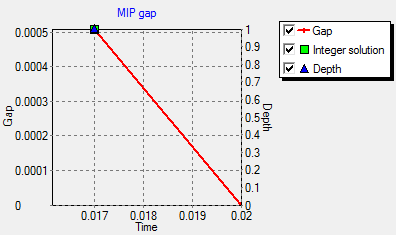
\includegraphics[scale=.8]{g1.png}
  \caption{MIP gap}
  \label{fig:sub1}
\end{subfigure}%
\begin{subfigure}{.5\textwidth}
  \centering
  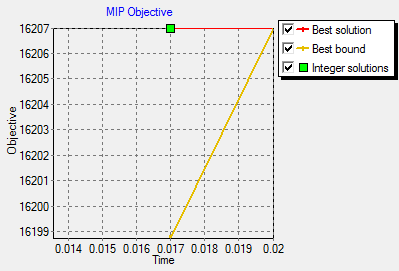
\includegraphics[scale=.7]{g2.png}
  \caption{MIP Objective}
  \label{fig:sub2}
\end{subfigure}
\caption{MIP Search for Conference Management} 
\label{fig:test}
\end{figure}

\begin{figure}[ht]
\centering
\begin{subfigure}{.5\textwidth}
  \centering
  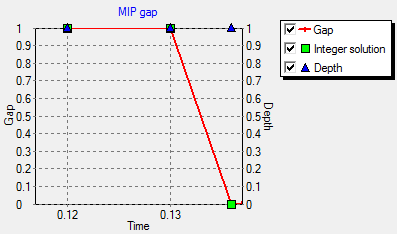
\includegraphics[scale=.8]{g3.png}
  \caption{MIP gap}
  \label{fig:sub1}
\end{subfigure}%
\begin{subfigure}{.5\textwidth}
  \centering
  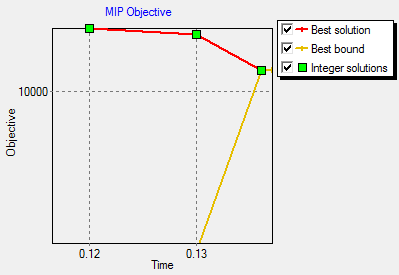
\includegraphics[scale=.7]{g4.png}
  \caption{MIP Objective}
  \label{fig:sub2}
\end{subfigure}
\caption{MIP Search for Expedia dataset } 
\label{fig:test}
\end{figure}

Scalability of this program has been tested on hotel property data, for that appropriate data cleansing and scaling is done  to generate data in required format. This dataset has 84 variables and each hotel is rated on the scale of 0 to 5 (0 is very poor,1 is poor, 2 is acceptable, 3 is good, 4 is very good and  5 is excellent). In this case, room will be allocated when average customer satisfaction rating is at least 3.3.\\

In fig 2(a) and fig 3(a) shows the evolution in time of the MIP gap during the global search and fig2(b) \& fig3(b) shows the progress of the current best integer solution objective relative to the best bound. For expedia data, integer solutions is found at three points. If we compare time for searching optimal solutions then Conference management found optimal solutions within 0.02 seconds and for expedia dataset best optimal solution is found within 0.13 seconds. Hence, Integer Linear programming take more time to solve if number of variables in the dataset increases gradually.\\

\textbf{Data Source:} Expedia Affiliate Network - Property Data \textit{URL: \url{http://developer.ean.com/database/property-data}} \\
\begin{verbatim}
!Expedia Hotel Property dataset
PRICE:[ 84,84,195,68,99,86,151,351,72,94,637,400,59,159,66,73,67,49,101,115,62,180,253,272,143,
86,55,61,67,135,40,171,140,122,140,435,75,118,35,70,204,180,108,237,184,140,107,100,262,109,327,
289,176,512,97,74,212,172,593,773,103,58,76,476,84,58,242,80,275,2425,57,75,87,87,55,29,359,143,
159,2603,80,128,101,229]	 	

RATING: [3,0,0,2.5,3,2.5,3,4,2.5,3,3.5,4,3,3.5,3,0,3,3.5,3,3,2.5,4,4.5,4,3.5,2.5,2,3,0,3,3,3,2.5,
3,3.5,4,0,3,2.5,2.5,3,0,0,0,2.5,3,2.5,3,4.5,2.5,2.5,3.5,3.5,3,0,3.5,3,0,0,3.5,3,3.5,0,3,2,3,4,
3.5,3.5,4,2.5,3,3,0,3.5,2,0,3,0,2.5,1,0,4,3.5]

AVAIL:[16,6,16,1,5,6,1,14,1,1,7,17,22,14,16,16,17,1,1,1,16,33,14,17,16,6,1,6,6,5,33,14,1,1,16,14,
16,1,1,2,1,14,5,16,1,1,1,1,16,1,22,1,14,5,5,16,14,6,16,14,16,1,1,1,1,6,1,11,1,17,32,1,1,16,6,12,4
,6,16,6,5,16,5,22] 
\end{verbatim}
%----------------------------------------------------------------------------------------
%	CONCLUSIONS
%----------------------------------------------------------------------------------------

\section{Conclusions}
\clearpage
\pagenumbering{roman}
\appendix{\LARGE{\textbf{Appendix}}}

\section{Code}
\begin{verbatim}
model Conference_Management
uses "mmxprs"; !gain access to the Xpress-Optimizer solver
	declarations
		HI = 1..10                       	! Index range
		PRICE: array(HI) of integer         ! Price table
		RATING: array(HI) of real			!Customer Satsifcation rating
		AVAIL: array(HI) of integer			!Available Rooms in a hotel
		decVar: array(HI) of mpvar          !Decision Variables
	end-declarations
	Max_Guest := 150
	
	!Read in the data from our text file
	initializations from 'Conference_Management.txt'
		PRICE
		RATING
		AVAIL
	end-initializations
	
	!procedure to check problem status
	procedure print_status
		declarations
			status: string
		end-declarations
		case getprobstat of
		XPRS_OPT: status:="LP Optimum found"
		XPRS_UNF: status:="Unfinished"
		XPRS_INF: status:="Infeasible"
		XPRS_UNB: status:="Unbounded"
		XPRS_OTH: status:="Failed"
		else status:="???"
		end-case
		writeln("Problem status: ", status)
	end-procedure
	 
	!Minimiz cost
	Cost:= sum(i in HI) PRICE(i)*decVar(i)
	 
	!Constraints
	!Declare that our decision variables are integers
	forall (i in HI) do 
		decVar(i) is_integer
	end-do
	
	AvgRating:= (sum(i in HI) RATING(i)*decVar(i))/150 >= 8.3
			 
	forall( i in HI)
		decVar(i) <= AVAIL(i)	 	
	sum(i in HI) decVar(i)	= Max_Guest
		
	!Display output of solution values
	procedure print_sol	
		writeln("Begin running model") 	
		writeln("---------------------------------------------------------")
		print_status
		writeln("Cost is: €",getobjval)
		writeln("---------------------------------------------------------")
		forall(i in HI) 
			writeln("Passenger in Hotel_",i," -> ", getsol(decVar(i)))
			
		!write value of AvgRating to output
		writeln(getsol(AvgRating))
		writeln("---------------------------------------------------------")
		exportprob(EP_MIN,"",Cost)
		writeln("---------------------------------------------------------")
		exportprob(1,"Conference_Management",Cost)
		writeln("End running model")
		!Modify Optimizer control parameter PSEUDOCOST
	end-procedure 
	minimize(Cost)
	print_sol	
end-model
\end{verbatim}
\section{Input and Output}
\subsection{Case 1: Original Data (10 Variables)}
\textbf{Input}
\begin{verbatim}
! Data file for `20. Conference Management Assignment - 2'

PRICE: [ 89, 99, 119, 112,143,94,130,98,155,152] !Constraint coefficients	 	

RATING: [7.8,8.3,8.0,8.7,8.0,8.1,8.6,8.9,8.9,8.4] !Constraint coefficients

AVAIL:[35,30,15,15,15,20,15,10,10,20] !Values of the constraints
\end{verbatim}
\textbf{Output}
\begin{verbatim}
Begin running model
---------------------------------------------------------
Problem status: LP Optimum found
Cost is: €16207
---------------------------------------------------------
Passenger in Hotel_1 -> 35
Passenger in Hotel_2 -> 30
Passenger in Hotel_3 -> 6
Passenger in Hotel_4 -> 15
Passenger in Hotel_5 -> 0
Passenger in Hotel_6 -> 20
Passenger in Hotel_7 -> 15
Passenger in Hotel_8 -> 10
Passenger in Hotel_9 -> 10
Passenger in Hotel_10 -> 9
0.000666667
---------------------------------------------------------
\ Using Xpress-MP extensions
Minimize
 89 decVar(1) + 99 decVar(2) + 119 decVar(3) + 112 decVar(4) + 143 decVar(5) + 
94 decVar(6) + 130 decVar(7) + 98 decVar(8) + 155 decVar(9) + 152 decVar(10)

Subject To
_R1: decVar(1) + decVar(2) + decVar(3) + decVar(4) + decVar(5) + decVar(6) + 
decVar(7) + decVar(8) + decVar(9) + decVar(10) = 150
AvgRating: 0.052 decVar(1) + 0.0553333 decVar(2) + 0.0533333 decVar(3) + 0.058 decVar(4) + 
0.0533333 decVar(5) + 0.054 decVar(6) + 0.0573333 decVar(7) + 0.0593333 decVar(8) + 
0.0593333 decVar(9) + 0.056 decVar(10) >= 8.3

Bounds
decVar(1) <= 35
decVar(2) <= 30
decVar(3) <= 15
decVar(4) <= 15
decVar(5) <= 15
decVar(6) <= 20
decVar(7) <= 15
decVar(8) <= 10
decVar(9) <= 10
decVar(10) <= 20

Integers
decVar(1) decVar(2) decVar(3) decVar(4) decVar(5) decVar(6) decVar(7) decVar(8) 
decVar(9) decVar(10) 

End
---------------------------------------------------------
End running model
\end{verbatim}

\subsection{Case 2: Scale Up to 20 Variables}
\textbf{Input}
\begin{verbatim}
! Data file for `20. Conference Management Assignment - 2'

PRICE: [ 89, 99, 119, 112,143,94,130,98,155,152,55,68,99,140,87,75,78,110,96,74] !Constraint coefficients	 	

RATING: [7.8,8.3,8.0,8.7,8.0,8.1,8.6,8.9,8.9,8.4,9.5,7.6,9.5,7.9,8.3,8.2,9.9,8.8,8.0,8.9] !Constraint coefficients

AVAIL:[35,30,15,15,15,20,15,10,10,20,2,5,6,7,9,1,2,5,4,6] !Values of the constraints
\end{verbatim}
\textbf{Output}
\begin{verbatim}
Begin running model
---------------------------------------------------------
Problem status: LP Optimum found
Cost is: €14061
---------------------------------------------------------
Passenger in Hotel_1 -> 35
Passenger in Hotel_2 -> 30
Passenger in Hotel_3 -> 0
Passenger in Hotel_4 -> 15
Passenger in Hotel_5 -> 0
Passenger in Hotel_6 -> 20
Passenger in Hotel_7 -> 0
Passenger in Hotel_8 -> 10
Passenger in Hotel_9 -> 0
Passenger in Hotel_10 -> 0
Passenger in Hotel_11 -> 2
Passenger in Hotel_12 -> 5
Passenger in Hotel_13 -> 6
Passenger in Hotel_14 -> 0
Passenger in Hotel_15 -> 9
Passenger in Hotel_16 -> 1
Passenger in Hotel_17 -> 2
Passenger in Hotel_18 -> 5
Passenger in Hotel_19 -> 4
Passenger in Hotel_20 -> 6
0.0306667
---------------------------------------------------------
\ Using Xpress-MP extensions
Minimize
 89 decVar(1) + 99 decVar(2) + 119 decVar(3) + 112 decVar(4) + 143 decVar(5) + 
94 decVar(6) + 130 decVar(7) + 98 decVar(8) + 155 decVar(9) + 152 decVar(10) + 
55 decVar(11) + 68 decVar(12) + 99 decVar(13) + 140 decVar(14) + 87 decVar(15) + 
75 decVar(16) + 78 decVar(17) + 110 decVar(18) + 96 decVar(19) + 74 decVar(20)

Subject To
_R1: decVar(1) + decVar(2) + decVar(3) + decVar(4) + decVar(5) + decVar(6) + 
decVar(7) + decVar(8) + decVar(9) + decVar(10) + decVar(11) + decVar(12) + decVar(13) + 
decVar(14) + decVar(15) + decVar(16) + decVar(17) + decVar(18) + decVar(19) + 
decVar(20) = 150
AvgRating: 0.052 decVar(1) + 0.0553333 decVar(2) + 0.0533333 decVar(3) + 0.058 decVar(4) + 
0.0533333 decVar(5) + 0.054 decVar(6) + 0.0573333 decVar(7) + 0.0593333 decVar(8) + 
0.0593333 decVar(9) + 0.056 decVar(10) + 0.0633333 decVar(11) + 0.0506667 decVar(12) + 
0.0633333 decVar(13) + 0.0526667 decVar(14) + 0.0553333 decVar(15) + 0.0546667 decVar(16) + 
0.066 decVar(17) + 0.0586667 decVar(18) + 0.0533333 decVar(19) + 0.0593333 decVar(20) >= 8.3

Bounds
decVar(1) <= 35
decVar(2) <= 30
decVar(3) <= 15
decVar(4) <= 15
decVar(5) <= 15
decVar(6) <= 20
decVar(7) <= 15
decVar(8) <= 10
decVar(9) <= 10
decVar(10) <= 20
decVar(11) <= 2
decVar(12) <= 5
decVar(13) <= 6
decVar(14) <= 7
decVar(15) <= 9
decVar(17) <= 2
decVar(18) <= 5
decVar(19) <= 4
decVar(20) <= 6

Integers
decVar(1) decVar(2) decVar(3) decVar(4) decVar(5) decVar(6) decVar(7) decVar(8) 
decVar(9) decVar(10) decVar(11) decVar(12) decVar(13) decVar(14) decVar(15) 
decVar(16) decVar(17) decVar(18) decVar(19) decVar(20) 

End
---------------------------------------------------------
End running model
\end{verbatim}



\subsection{Case 2: Scale Up to 20 Variables}
\textbf{Input}
\begin{verbatim}
! Data file for `20. Conference Management Assignment 2'

PRICE: [ 89, 99, 119, 112,143,94,130,98,155,152,55,68,99,140,87,75,78,110,96,74,65,5,40,30,30,17,15,89,10,20] !Constraint coefficients	 	

RATING: [7.8,8.3,8.0,8.7,8.0,8.1,8.6,8.9,8.9,8.4,9.5,7.6,9.5,7.9,8.3,8.2,9.9,8.8,8.0,8.9,8.1,8.3,8.2,8.5,8.9,9.5,7.8,9.1,8.1,8.2] !Constraint coefficients

AVAIL:[35,30,15,15,15,20,15,10,10,20,2,5,6,7,9,1,2,5,4,6,2,5,4,6,1,2,3,17,2,5] !Values of the constraints
\end{verbatim}
\textbf{Output}
\begin{verbatim}
Begin running model
---------------------------------------------------------
Problem status: LP Optimum found
Cost is: €11395
---------------------------------------------------------
Passenger in Hotel_1 -> 35
Passenger in Hotel_2 -> 3
Passenger in Hotel_3 -> 0
Passenger in Hotel_4 -> 0
Passenger in Hotel_5 -> 0
Passenger in Hotel_6 -> 20
Passenger in Hotel_7 -> 0
Passenger in Hotel_8 -> 10
Passenger in Hotel_9 -> 0
Passenger in Hotel_10 -> 0
Passenger in Hotel_11 -> 2
Passenger in Hotel_12 -> 5
Passenger in Hotel_13 -> 6
Passenger in Hotel_14 -> 0
Passenger in Hotel_15 -> 9
Passenger in Hotel_16 -> 1
Passenger in Hotel_17 -> 2
Passenger in Hotel_18 -> 0
Passenger in Hotel_19 -> 4
Passenger in Hotel_20 -> 6
Passenger in Hotel_21 -> 2
Passenger in Hotel_22 -> 5
Passenger in Hotel_23 -> 4
Passenger in Hotel_24 -> 6
Passenger in Hotel_25 -> 1
Passenger in Hotel_26 -> 2
Passenger in Hotel_27 -> 3
Passenger in Hotel_28 -> 17
Passenger in Hotel_29 -> 2
Passenger in Hotel_30 -> 5
0.0713333
---------------------------------------------------------
\ Using Xpress-MP extensions
Minimize
 89 decVar(1) + 99 decVar(2) + 119 decVar(3) + 112 decVar(4) + 143 decVar(5) + 
94 decVar(6) + 130 decVar(7) + 98 decVar(8) + 155 decVar(9) + 152 decVar(10) + 
55 decVar(11) + 68 decVar(12) + 99 decVar(13) + 140 decVar(14) + 87 decVar(15) + 
75 decVar(16) + 78 decVar(17) + 110 decVar(18) + 96 decVar(19) + 74 decVar(20) + 
65 decVar(21) + 5 decVar(22) + 40 decVar(23) + 30 decVar(24) + 30 decVar(25) + 
17 decVar(26) + 15 decVar(27) + 89 decVar(28) + 10 decVar(29) + 20 decVar(30)

Subject To
_R1: decVar(1) + decVar(2) + decVar(3) + decVar(4) + decVar(5) + decVar(6) + 
decVar(7) + decVar(8) + decVar(9) + decVar(10) + decVar(11) + decVar(12) + decVar(13) + 
decVar(14) + decVar(15) + decVar(16) + decVar(17) + decVar(18) + decVar(19) + 
decVar(20) + decVar(21) + decVar(22) + decVar(23) + decVar(24) + decVar(25) + 
decVar(26) + decVar(27) + decVar(28) + decVar(29) + decVar(30) = 150
AvgRating: 0.052 decVar(1) + 0.0553333 decVar(2) + 0.0533333 decVar(3) + 0.058 decVar(4) + 
0.0533333 decVar(5) + 0.054 decVar(6) + 0.0573333 decVar(7) + 0.0593333 decVar(8) + 
0.0593333 decVar(9) + 0.056 decVar(10) + 0.0633333 decVar(11) + 0.0506667 decVar(12) + 
0.0633333 decVar(13) + 0.0526667 decVar(14) + 0.0553333 decVar(15) + 0.0546667 decVar(16) + 
0.066 decVar(17) + 0.0586667 decVar(18) + 0.0533333 decVar(19) + 0.0593333 decVar(20) + 
0.054 decVar(21) + 0.0553333 decVar(22) + 0.0546667 decVar(23) + 0.0566667 decVar(24) + 
0.0593333 decVar(25) + 0.0633333 decVar(26) + 0.052 decVar(27) + 0.0606667 decVar(28) + 
0.054 decVar(29) + 0.0546667 decVar(30) >= 8.3

Bounds
decVar(1) <= 35
decVar(2) <= 30
decVar(3) <= 15
decVar(4) <= 15
decVar(5) <= 15
decVar(6) <= 20
decVar(7) <= 15
decVar(8) <= 10
decVar(9) <= 10
decVar(10) <= 20
decVar(11) <= 2
decVar(12) <= 5
decVar(13) <= 6
decVar(14) <= 7
decVar(15) <= 9
decVar(17) <= 2
decVar(18) <= 5
decVar(19) <= 4
decVar(20) <= 6
decVar(21) <= 2
decVar(22) <= 5
decVar(23) <= 4
decVar(24) <= 6
decVar(26) <= 2
decVar(27) <= 3
decVar(28) <= 17
decVar(29) <= 2
decVar(30) <= 5

Integers
decVar(1) decVar(2) decVar(3) decVar(4) decVar(5) decVar(6) decVar(7) decVar(8) 
decVar(9) decVar(10) decVar(11) decVar(12) decVar(13) decVar(14) decVar(15) 
decVar(16) decVar(17) decVar(18) decVar(19) decVar(20) decVar(21) decVar(22) 
decVar(23) decVar(24) decVar(25) decVar(26) decVar(27) decVar(28) decVar(29) 
decVar(30) 

End
---------------------------------------------------------
End running model

\end{verbatim}
\bibliographystyle{agsm}
\addcontentsline{toc}{section}{References} 
\end{document}

